% Rescaling the vertical direction by an analytically-varying (linear) factor: still the same line bundle structure.
% Source: book/tex/riemann-surface/line-bundles.tex (asy figure).
\documentclass[border=2mm]{standalone}
\usepackage{tikz}
\begin{document}
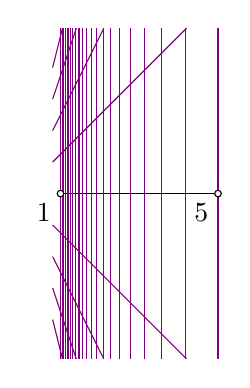
\begin{tikzpicture}[scale=0.5,>=latex]
  \draw (1,0) -- (5,0);
  \node[anchor=north east] at (1,0) {$1$};
  \node[anchor=north east] at (5,0) {$5$};
  \draw[violet] (5.0000,-4.2) -- (5.0000,4.2);
  \draw[violet] (4.1667,-4.2) -- (4.1667,4.2);
  \draw[violet] (3.5714,-4.2) -- (3.5714,4.2);
  \draw[violet] (3.1250,-4.2) -- (3.1250,4.2);
  \draw[violet] (2.7778,-4.2) -- (2.7778,4.2);
  \draw[violet] (2.5000,-4.2) -- (2.5000,4.2);
  \draw[violet] (2.2727,-4.2) -- (2.2727,4.2);
  \draw[violet] (2.0833,-4.2) -- (2.0833,4.2);
  \draw[violet] (1.9231,-4.2) -- (1.9231,4.2);
  \draw[violet] (1.7857,-4.2) -- (1.7857,4.2);
  \draw[violet] (1.6667,-4.2) -- (1.6667,4.2);
  \draw[violet] (1.5625,-4.2) -- (1.5625,4.2);
  \draw[violet] (1.4706,-4.2) -- (1.4706,4.2);
  \draw[violet] (1.3889,-4.2) -- (1.3889,4.2);
  \draw[violet] (1.3158,-4.2) -- (1.3158,4.2);
  \draw[violet] (1.2500,-4.2) -- (1.2500,4.2);
  \draw[violet] (1.1905,-4.2) -- (1.1905,4.2);
  \draw[violet] (1.1364,-4.2) -- (1.1364,4.2);
  \draw[violet] (1.0870,-4.2) -- (1.0870,4.2);
  \draw[violet] (1.0417,-4.2) -- (1.0417,4.2);
  \draw[violet] (1.0000,-4.2) -- (1.0000,4.2);
  \draw[violet] (0.8,0.8000) -- (4.2000,4.2000);
  \draw[violet] (0.8,-0.8000) -- (4.2000,-4.2000);
  \draw[violet] (0.8,1.6000) -- (2.1000,4.2000);
  \draw[violet] (0.8,-1.6000) -- (2.1000,-4.2000);
  \draw[violet] (0.8,2.4000) -- (1.4000,4.2000);
  \draw[violet] (0.8,-2.4000) -- (1.4000,-4.2000);
  \draw[violet] (0.8,3.2000) -- (1.0500,4.2000);
  \draw[violet] (0.8,-3.2000) -- (1.0500,-4.2000);
  \filldraw[fill=white] (1,0) circle (2.4pt);
  \filldraw[fill=white] (5,0) circle (2.4pt);
\end{tikzpicture}
\end{document}
